\documentclass[a4paper, margin=1in]{article}
%\usepackage{CJK}
\usepackage{latexsym}
\usepackage{color}
\usepackage[x11names]{xcolor} % for a set of predefined color names, like LemonChiffon1
\usepackage{graphicx, float}\usepackage{graphicx}
\usepackage{algorithmic}
\usepackage{algorithm}
%\usepackage{algpseudocode}
%\usepackage[colorlinks]{hyperref}
\usepackage[toc,page]{appendix}
\usepackage{bm}
\setlength{\oddsidemargin}{-0.0in}
\setlength{\evensidemargin}{-0.0in} \setlength{\textwidth}{6.0in}
\setlength{\textheight}{9.0in} \setlength{\topmargin}{-0.2in}
%\usepackage[boxruled]{algorithm2e}

%\setlength{\leftmargin}{0.7in}
\usepackage{amssymb, graphicx, amsmath}  %  fancyheadings,
\usepackage{setspace}
\newcommand\qed{\qquad $\square$}
\newcommand{\nn}{\nonumber}

\usepackage{lipsum}

\usepackage{listings}
\lstset{
  basicstyle=\ttfamily,
  columns=fullflexible,
  frameround=fttt,
  breaklines=true,
  %postbreak=\mbox{\textcolor{red}{$\hookrightarrow$}\space},
}

\definecolor{mGreen}{rgb}{0,0.6,0}
\definecolor{mGray}{rgb}{0.5,0.5,0.5}
\definecolor{mPurple}{rgb}{0.58,0,0.82}
\definecolor{backgroundColour}{rgb}{0.95,0.95,0.92}

\lstdefinestyle{CStyle}{
basicstyle=\ttfamily,
language=C,
numberstyle=\tiny\color{mGray},
numbers=left,
frame=lines,
framexleftmargin=0.5em,
framexrightmargin=0.5em,
backgroundcolor=\color{LemonChiffon1},
showstringspaces=false,
escapeinside={(*@}{@*)},
}

\def \[{\begin{equation}}
\def \]{\end{equation}}
\def\proof{{\bf Proof:\quad}}
\def \endzm {\quad $\Box$}
\def\dist{\hbox{dist}}

\usepackage{tabularx,booktabs}
\newcolumntype{C}{>{\centering\arraybackslash\hsize=.5\hsize}X} % centered version of "X" type
\setlength{\extrarowheight}{1pt}
\usepackage{caption}% <-- added


\newcommand{\R}{\mathbb{R}}
%\newtheorem{yinli}{����}[section]
\newcommand{\D}{\displaystyle}
\newcommand{\T}{\textstyle}
\newcommand{\SC}{\scriptstyle}
\newcommand{\FT}{\footnotesize}

\usepackage{hyperref}
\newcommand\fnurl[2]{%
  \href{#2}{#1}\footnote{\url{#2}}%
}


%\newtheorem{theorem}{Theorem}[section]
%\renewcommand{\thetheorem}{\arabic{section}.\arabic{theorem}}
\newtheorem{definition}{Definition}
\renewcommand{\thedefinition}{\arabic{section}.\arabic{definition}}
\newtheorem{lemma}{Lemma}[section]
\renewcommand{\thelemma}{\arabic{section}.\arabic{lemma}}
\newtheorem{remark}{Remark}
\renewcommand{\theremark}{\arabic{section}.\arabic{remark}}
\newtheorem{proposition}{Proposition}[section]
\renewcommand{\theproposition}{\arabic{section}.\arabic{proposition}}
\newtheorem{corollary}{Corollary }[section]
\renewcommand{\thecorollary}{\arabic{section}.\arabic{corollary}}
\renewcommand{\theequation}{\arabic{section}.\arabic{equation}}
\renewcommand{\baselinestretch}{1.35}
\newtheorem{exam}{Example}[section]
\renewcommand{\theexam}{\arabic{section}.\arabic{exam}}
\newtheorem{theo}{Theorem}[section]
\renewcommand{\thetheo}{\arabic{section}.\arabic{theo}}

\usepackage{enumitem}
\newenvironment{QandA}{\begin{enumerate}[label=\bfseries\alph*.]\bfseries}
	{\end{enumerate}}
\newenvironment{answered}{\par\normalfont}{}

% Define a \HEADER{Title} ... \ENDHEADER block
\makeatletter
\newcommand{\HEADER}[1]{\ALC@it\underline{\textsc{#1}}\begin{ALC@g}}
\newcommand{\ENDHEADER}{\end{ALC@g}}
\makeatother

\newcommand{\argmin}{\operatornamewithlimits{argmin}}
\newcommand{\argmax}{\operatornamewithlimits{argmax}}

\usepackage{url} % to make url in bibtex shows up

% Create a command to cleanly insert a snippet with the style above anywhere in the document
\newcommand{\insertcode}[2]{\begin{itemize}\item[]\lstinputlisting[caption=#2,label=#1,style=CStyle]{#1}\end{itemize}} % The first argument is the script location/filename and the second is a caption for the listing

\begin{document}
%\begin{CJK*}{GBK}{song}

\begin{center}

{\LARGE \bf CS380L: Advanced Operating Systems Lab \#2}\\

\vskip 25pt
 {Zeyuan Hu \footnote{30 hours spent on this lab.}, iamzeyuanhu@utexas.edu }\\
\vskip 5pt
{\small EID:zh4378 Spring 2019 }

\end{center}

\begin{spacing}{1.5}
\section{Environment} \label{environment}

We have two Linux machines for experiments: \texttt{erode-lom} and \texttt{thoothukudi-lom}. Both of them run Ubuntu 16.04 LTS. \footnote{\texttt{erode-lom} with ip address: \lstinline|192.168.1.120| and \texttt{thoothukudi-lom} with ip address: \texttt{192.168.1.121}. Due to the network setup, those two machines are not properly registered in the department DNS server. We use ip address instead host names to logon these two machines.}

\section{System Tools Exercise}

\subsection{strace}

\texttt{script} command allows user to record terminal printout into a file \cite{script_man}. Per the lab instruction, we use \texttt{strace} to trace the syscalls and signals of a target process \cite{strace_man}. In our case, we trace the process involving \texttt{cat}. One thing I notice is that \texttt{script} contains some unicode as shown in Figure \ref{session}. Thus, we use the following code to clean up the output:

\begin{lstlisting}[style=CStyle]
cat $FILE | perl -pe 's/\e([^\[\]]|\[.*?[a-zA-Z]|\].*?\a)//g' | col -b > $FILE-processed
\end{lstlisting}

The result is shown in Figure \ref{session_processed} \footnote{raw output and cleanup output comes with the report as \texttt{session\_record} and 
\texttt{session\_record-processed} respectively}. 

\begin{figure}
	\centering
	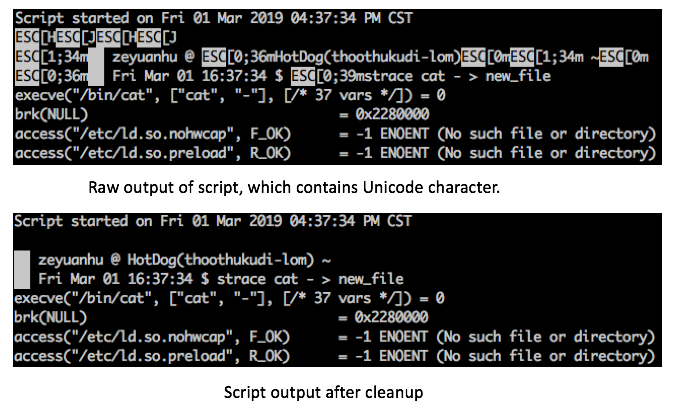
\includegraphics[scale=0.5]{session_record.png} 
	\caption{\texttt{script} output before and after cleanup}
	\label{session_processed}
\end{figure}

\subsection{lsof}

\texttt{lsof} lists all open files \cite{lsof_man}. \texttt{lsof | grep /dev} shows all the open devices used by user-space programs. On our machine, we have the following opened devices:

\begin{itemize}
	\item \texttt{/dev/null}: null device
	\item \texttt{/dev/pts/*} and \texttt{/dev/tty}: terminal devices
	\item \texttt{/dev/urandom}:  kernel random number source device
	\item \texttt{/dev/ptmx}: a character file to create a pseudoterminal master
\end{itemize}

\section{Network Tools}

\texttt{ifconfig} command lists all the network interfaces the machine is using to communicate externally. On our machine, interface for Ethernet is \texttt{eno1}. We can find IP address, gateway address, and subnet mask from the output.

\texttt{tcpdump} command can dump traffic on a network interface.  We use the \texttt{tcpdump} output provided by the lab instruction to answer the questions below.

\begin{QandA}
	\item Are DHCP messages sent over UDP or TCP?
	\begin{answered}
	We use \lstinline!tcpdump -nn -r tcpdump.out.1 | grep -i dhcp! to filter out the DHCP messages from the dump. \lstinline|-nn| ensures that we can see the actual port number instead of the port name. One line of the output is: 
	\begin{lstlisting}
10:19:24.525962 IP 0.0.0.0.68 > 255.255.255.255.67: BOOTP/DHCP, Request from a8:20:66:3b:66:51, length 300
	\end{lstlisting}
	The first field shows the time that the packet was traveling. The second field shows the source host address and port, followed by the destination host address and port. The third field shows the protocl the packet was using. From DHCP \cite{dhcp}, we know DHCP messages sent over UDP. As shown by the printout, the messages are sent between port 68 (client) and port 67 (server).
	\end{answered}
	
	\item What is the link-layer (e.g., Ethernet) address of your host? (Feel free to obscure the last couple bytes for privacy's sake)
	\begin{answered}
	We use the same \texttt{tcpdump} command as above with extra \texttt{-e} option to show linke-layer header. The following printout contains DHCP messages for acquiring IP address:
	\begin{lstlisting}
10:19:24.525962 a8:20:66:3b:66:51 > ff:ff:ff:ff:ff:ff, ethertype IPv4 (0x0800), length 342: 0.0.0.0.68 > 255.255.255.255.67: BOOTP/DHCP, Request from a8:20:66:3b:66:51, length 300
10:19:24.566258 00:21:9b:fb:61:0c > a8:20:66:3b:66:51, ethertype IPv4 (0x0800), length 342: 128.83.158.2.67 > 128.83.158.160.68: BOOTP/DHCP, Reply, length 30
	\end{lstlisting}
	From the printout we can see that the link-layer address (MAC address) of the host is \texttt{a8:20:66:3b:66:51}.
	\end{answered}

	\item What is the IP address of your DHCP server?
	\begin{answered}
		From the printout above, we can see the IP address of DHCP server is 
		\lstinline|128.83.158.2| and the new IP address acquired from DHCP server is \lstinline|128.83.158.160|.
	\end{answered}

	\item What is the purpose of the DHCP release message? 
	\begin{answered}
		DHCP release message is used to release IP address.
	\end{answered}

	\item Does the DHCP server issue an acknowledgment of receipt of the client's DHCP request?
	\begin{answered}
		DHCP server does not issue an acknowledgment of receipt of the client?s release message.
	\end{answered}

	\item What would happen if the client's DHCP release message is lost?
	\begin{answered}
		 If DHCP release message is lost, the DHCP server has to wait for the lease to timeout before assigning it to other clients.
	\end{answered}
\end{QandA}

\section{User-level File System} 


\section{Measuring memory access behavior}

\texttt{mmap} system call maps files or devices into memory. The created mapping can be file-backed or anonymous. File-backed mapping maps an area of the process's virtual memory to files (i.e., an area of the process's virtual memory is mapped to file-backed memory); reading those areas of memory causes the file read. Anonymous mapping is the opposite of file-backed mapping (i.e., not backed by file; an area of the process's virtual memory is mapped to anonymous memory). In this section, we experiment with both types of mappings. Since file-backed mapping can be shared or private, we have three memory mappings setup in our experiment: anonymous, file-based (private) and file-based (share).
In this experiment, we use \lstinline|MAP_POPULATE| flag. \lstinline|MAP_POPULATE| populates page tables for a mapping. For file-backed mapping, this means read-ahead on file, which reduce blocking on page faults later. In addition, we use \texttt{memset} to initialize the mapped region and \texttt{msync} to flush the change made to the file-backed memory back to file system whenever possible. 

We study the following code, which is used to access the mapped region:

\begin{lstlisting}[style=CStyle]
#define CACHE_LINE_SIZE 64
int opt_random_access;  
void do_mem_access(char *p, int size) {
  int outer, locality, i;
  int ws_base = 0;
  int max_base = size / CACHE_LINE_SIZE - 512;
  for (outer = 0; outer < (1 << 20); outer++) {
    long r = simplerand() % max_base;
    if (opt_random_access) {
      ws_base = r;
    } else {
      ws_base += 512;
      if (ws_base >= max_base) {
        ws_base = 0;
      }
    }
    for (locality = 0; locality < 16; locality++) {
      volatile char *a;
      char c;
      for (i = 0; i < 512; i++) {
        a = p + ws_base + i * CACHE_LINE_SIZE;
        if (i % 8 == 0) {
          *a = 1;
        } else {
          c = *a;
        }
      }
    }
  }
}
\end{lstlisting}

\lstinline|simplerand()| is a function generates random number. A global variable \lstinline|opt_random_access| is used to specify the
memory access to be sequential or random. Specifically, \lstinline|db_mem_access()| routine will access a working set consists of
512 consecutive cache lines. Among those 512 cache lines, $\frac{1}{8}$ will be write access and $\frac{7}{8}$ will be read access. The
same working set is accessed 16 times. The whole routine will work on $2^{20}$ working sets. Working sets are selected either sequentially
or in random (specified by \lstinline|opt_random_access|). In sequential access case, offset between working sets is 512 (e.g., since there
are 512 cache lines of a set). In random access case, the start(i.e., base) of working set is selected randomly based on the number generated by \lstinline|simplerand()|. \lstinline|simplerand()| is called no matter the sequential memory access or random access because we want to keep the
experiment results difference only due to the memory access pattern difference. In other words, we want to have both memory access patterns have the same function call and context switch overheads (caused by calling \lstinline|simplerand()|).

We study \lstinline|db_mem_access()| behavior on a VM with 2GB of memory and 4 virtual CPU cores. The VM runs Ubuntu 18.10 with kernel version 4.19.6. \lstinline|-cpu host| is added as part of QEMU option to ensure our VM can access performance counters. We allocate 1GB buffer via \texttt{mmap} as input for \lstinline|do_mem_access|.  To ensure 
the repeatable result, we flush the level 1 data cache by accessing a 16MB buffer before calling \lstinline|do_mem_access|. We invoke \texttt{getrusage}  just before and after \lstinline|do_mem_access| to collect resource usage statistics of initialization code and \lstinline|do_mem_access|. We run the program 5 times and calculate mean and stand deviation of statistics \footnote{We compile our program with \texttt{-O2} to prevent any unwanted memory access from the generated executable}. We also submit the raw results along with this report.

\begin{figure}	
	\centering
	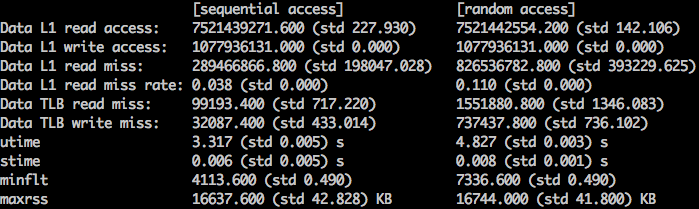
\includegraphics[scale=0.65]{sequential_random_anonymous} 
	\caption{The statistics of sequential and random memory accesses with anonymous mapped memory regions}
	\label{sequential_random_anonymous}
\end{figure}

We first compare sequential access and random access (indicated by \lstinline|opt_random_access|). We use anonymous mapped memory regions. Figure \ref{sequential_random_anonymous} shows  statistics for both cases \footnote{\texttt{majflt}, \texttt{inblock}, \texttt{oublock} are omitted because they are all 0}.  As shown in the figure, the ratio between read and write access is 7:1 for data L1 cache for both cases, which is as expected. The read miss rate in random access case is 3x higher than sequential access. For data TLB, read miss and write miss of random access is 15.6X and 23x higher than sequential access respectively. Random access runs 1.46x slower than sequential access. From those statistics, we can see that there is no significant difference in terms of runtime and miss rate of data L1 cache between random access and sequential access (e.g., miss rate for random access is around 0.1). In the case of sequential access, the number of data TLB read miss is about 99193, which is
396MB for 4KB page size. 396MB is smaller than the size of our buffer. If we take a look at the code, we notice \lstinline|max_base| in \lstinline|do_mem_access| restricts the maximum base address of the working set. If we take a look at how \lstinline|max_base| is initialized and the line we initialize \texttt{a}, we can see that the working set is essentially the first $\frac{1}{64}$ of the given buffer, which is 16MB, which matches with the value of \texttt{maxrss} we observed and is much lower than 1GB. Realizing this fact also explains why TLB miss count is lower than the total number of data pages \footnote{If we want to access all the allocated buffer (1GB), we should replace line 21 (\texttt{a} initialization) with \lstinline|a = p + (ws_base + i) * CACHE_LINE_SIZE;| }.

\begin{figure}	
	\centering
	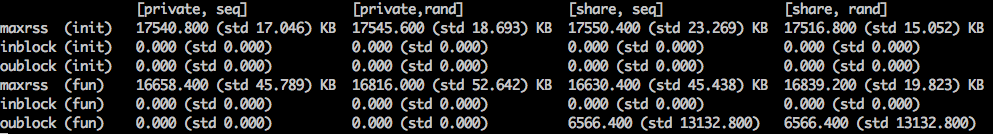
\includegraphics[scale=0.5]{share_private} 
	\caption{The statistics of sequential and random memory accesses with file-backed mapping with \lstinline|MAP_PRIVATE| and \lstinline|MAP_SHARED|. \texttt{fun} is a shorthand for \lstinline|do_mem_access|.}
	\label{share_private}
\end{figure}

In the next step, we experiment with file-based memory mappings.  In this part,
we only concern \texttt{maxrss}, \texttt{inblock}, and \texttt{oublock} because
the statistics related to data L1 cache and data TLB are generated with the same setup as anonymous mappings. In addition, statistics related to memory cache is not affected by the file-backed mapping. The statistics we have is shown in Figure \ref{share_private}. Compare to previous result, we notice there are 
large amount of \texttt{oublock} during \lstinline|do_mem_access| for file-backed mapping with \lstinline|MAP_SHARED|. This is intuitive as the changes to the file
have to be saved in shared mode. We notice that there is \texttt{inblock} is zero, 
which is due to the internal cache in Linux kernel for reading file.  \texttt{oublock} for both random access and sequential access under shared mode are exactly the same.  This may due to the fact that access pattern is not
significant for the shared mode as synchronization for internal file cache is needed no matter what memory access pattern we may encounter.

\begin{figure}	
	\centering
	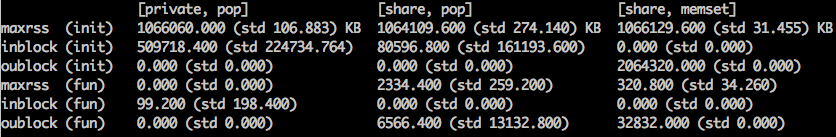
\includegraphics[scale=0.5]{populate_memset} 
	\caption{The statistics of file-backed mapping for \lstinline|MAP_POPULATE| and memset after buffer allocation. \texttt{fun} is a shorthand for \lstinline|do_mem_access|.}
	\label{populate_memset}
\end{figure}

In this experiment, we further examine \lstinline{MAP_POPULATE} flag and \texttt{memset} the mapped memory for initialization. Figure \ref{populate_memset} shows the statistics. Note that all the columns are from
the sequential memory access. With \lstinline|MAP_POPULATE| flag, the mapped memory will be populate page tables at the very beginning and perform read-ahead on the file. Thus we see the \texttt{maxrss} will match the allocated buffer size, which is around 1GB during the initialization. If the mapped memory 
is initialized with \texttt{memset} and then perform synchronization to the file system via \texttt{msync}, then there will be large amount of \texttt{oublock} during the initialization.

We also using \texttt{strace} to trace our program \footnote{we trace our program as \lstinline|strace ./memory_access 0 0 0 0 0 0|, where \lstinline|memory_access| is the executable from \lstinline|memory_access.c|}.  We find a system call \lstinline|arch_prctl(ARCH_SET_FS, 0x7f83a006d540) | in the printout. The system call means setting FS register to \texttt{0x7f83a006d540} \cite{arch_prctl_man}. FS register is a segment register with no specific processor-defined purpose and is given purpose by the OS. In Linux, FS register is for thread local storage. We can also see the system call \lstinline|access("/etc/ld.so.preload", R_OK)|, which tries to access \lstinline|/etc/ld.so.preload| file. This file contains ELF shared
objects, which are loaded before the execution of the program \cite{ld.so_man}. From the printout, we can see that this file is accessed before \texttt{libc.so} is loaded.

\section{Measuring memory access behavior with background activity}

In this section, we study the memory access behavior when there is a background activity. We use another process to allocate and access a large amount of memory to simulate background activity. We use \lstinline|compete_for_memory| function for this purpose.

\begin{lstlisting}[style=CStyle]
int compete_for_memory(void *unused) {
      long mem_size = get_mem_size();
      int page_sz = sysconf(_SC_PAGE_SIZE);
      printf(``Total memsize is %3.2f GBs\n'',
      (double)mem_size / (1024 * 1024 * 1024));
      fflush(stdout);
      char *p = mmap(NULL, mem_size, PROT_READ | PROT_WRITE,
      MAP_NORESERVE | MAP_PRIVATE | MAP_ANONYMOUS, -1, 0);
      if (p == MAP_FAILED) {
        perror(``Failed anon MMAP competition'');
        fflush(stdout);
        exit(EXIT_FAILURE);
      }

      int i = 0;
      while (1) {
        volatile char *a;
        long r = simplerand() % (mem_size / page_sz);
        char c;
        if (i >= mem_size / page_sz) {
          i = 0;
        }
        a = p + r * page_sz;
        c += *a;
        if (i % 8 == 0) {
          *a = 1;
        }
        i++;
      }
      return 0;
}
\end{lstlisting}

\lstinline|get_mem_size| is used to obtain the total amount of RAM of current system in bytes by reading from \texttt{/proc/meminfo} file. In the function above,
\lstinline|fflush(stdout)| is invoked after printing total memory. This is necessary because otherwise we cannot see the total memory message.  However, flush to stderr is not necessary because each print call to stderr will be automatically followed by a flush. Since \lstinline|compete_for_memory| function will try to allocate a memory region equals to the size of RAM, we need to setup swap file for the system because otherwise, the process will be killed due to oversubscribe of the memory. In the experiment, we setup a swap file of 2GB in the VM. \lstinline|compete_for_memory| is called by a separate child process via \texttt{fork}. The child process will be killed when the main process exits. After forking the child process, the main process will sleep for 5 seconds to wait for child process to allocate memory. The statistics is shown in Figure \ref{compete}. 
Note that the statistics is for anonymous mapping with random memory access. For other mapping and access behaviors, we submit the raw data along with the report. With memory pressure in the system, we expect the program takes more time to finish and encounters more page faults. From the statistics, we see that the program with memory pressure takes more time to finish and page faults are significantly higher than the no-compete case (shown both from \texttt{minflt} and \texttt{majflt}). However, read miss for both L1 cache and data TLB in compete case is slightly higher than the no-compete case.  We also see there are non-zero values of \texttt{inblock} in the case of memory pressure. This is another indicator that more page faults happened.  Other mappings (file-backed in shared and private mode) has similar statistics with slight higher page faults.

\begin{figure*}[!b]	
	\centering
	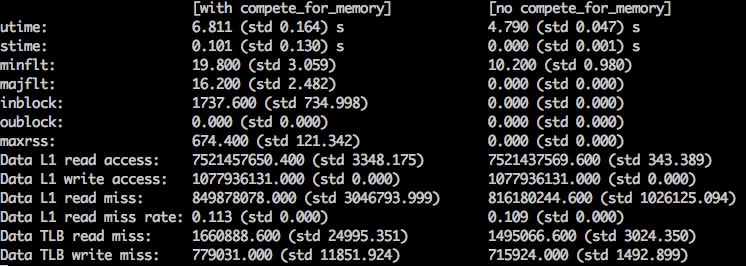
\includegraphics[scale=0.5]{compete} 
	\caption{The statistics of anonymous mapping for random memory access both with and without memory pressure}
	\label{compete}
\end{figure*}

Next, we modify the page replacement policy of Linux kernel. Linux kernel uses LRU to reclaim pages. We modify \lstinline|shrink_page_list| function in \lstinline|mm/vmscan.c| file. The target code block looks like below:

\begin{lstlisting}[style=CStyle]
switch (references) {
case PAGEREF_ACTIVATE:
                goto activate_locked;
case PAGEREF_KEEP:
                nr_ref_keep++;
                goto keep_locked;
case PAGEREF_RECLAIM:
case PAGEREF_RECLAIM_CLEAN:
                 ; /* try to reclaim the page below */
}
\end{lstlisting}

\begin{figure*}
	\centering
	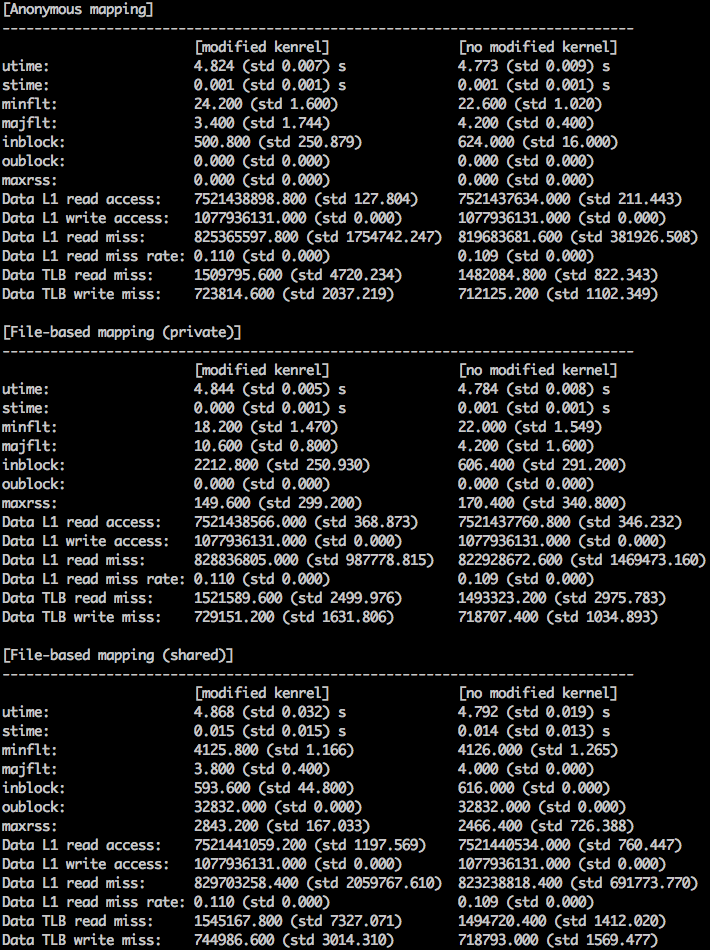
\includegraphics[scale=0.6]{modified} 
	\caption{The statistics of memory random access behavior under different mappings before and after the modification of the kernel}
	\label{modified}
\end{figure*}

We modify the \lstinline|PAGEREF_ACTIVATE| case to behave the same as \lstinline|PAGEREF_RECLAIM| case. Before the modification, \lstinline|PAGEREF_ACTIVATE| represents the case where the kernel sees the page has been recently accessed. Thus, the page will  not be swapped out of RAM. If we change this case to behave the same as \lstinline|PAGEREF_RECLAIM|, there is no LRU in the page replacement process. 
We conduct our experiment for memory random access under memory pressure for all possible mappings. The statistics is shown in Figure \ref{modified}. As one can see, since we disable the LRU replacement policy, the page faults increase in the modified kernel case. This is intuitive as the kernel might swap out pages that are frequently accessed.  However, we should note that the page faults do not increase dramatically as in theory LRU can behave worse than the no replacement policy at all especially when the memory access pattern is random. This is because random memory access may create some access pattern that is in favor of no replacement policy at all case. For example, there is a clear page faults increase for file-backed mapping in private mode. However, for anonymous mapping, page faults actually decrease after the modification. In addition, since the \lstinline|do_mem_access| frequently accesses around 16MB of memory, while the competing process uniformly accesses  its 2GB memory, the chance that a hot page being swapped out is relative small.



\end{spacing}
\bibliographystyle{ieeetr}
\bibliography{report}
\end{document}

